\documentclass{beamer}
\usepackage{fancyvrb}
\usepackage{hyperref}
\usepackage{multicol}
\usepackage{graphicx}
\usepackage{xcolor}
\newtheorem{theo}{Theorem}[section]

\newcommand{\myfig}[1]{\centerline{\includegraphics[scale=0.25]{figures/#1.png}}}

\newcommand{\trans}[5]{
\begin{tabular}{|c|c|c|c|c|}\hline
#1 & #2 & #3 & #4 & #5 \\\hline
\end{tabular}
}

\newcommand{\arr}{&\rightarrow&}
\newcommand{\darr}{&\Rightarrow&}
\newcommand{\ar}{\rightarrow}
\newcommand{\dar}{\Rightarrow}
\newcommand{\bee}{\begin{eqnarray*}}
\newcommand{\eee}{\end{eqnarray*}}
\newcommand{\lmb}{\ensuremath{\lambda}}

\newcommand{\bi}{\begin{itemize}}
\newcommand{\ii}{\item}
\newcommand{\ei}{\end{itemize}}

\newcommand{\sect}[1]{
\section{#1}
\begin{frame}[fragile]\frametitle{#1}
}

\mode<presentation>
{
%  \usetheme{Madrid}
  % or ...

%  \setbeamercovered{transparent}
  % or whatever (possibly just delete it)
}

\usepackage[english]{babel}

\usepackage[latin1]{inputenc}

\title
{
Scheme Notes 03
}

\subtitle{
} % (optional)

\author[Geoffrey Matthews]
{Geoffrey Matthews}
% - Use the \inst{?} command only if the authors have different
%   affiliation.

\institute[WWU/CS]
{
  Department of Computer Science\\
  Western Washington University
}
% - Use the \inst command only if there are several affiliations.
% - Keep it simple, no one is interested in your street address.

\date{\today}

% If you have a file called "university-logo-filename.xxx", where xxx
% is a graphic format that can be processed by latex or pdflatex,
% resp., then you can add a logo as follows:

%\pgfdeclareimage[height=0.5cm]{university-logo}{WWULogoProColor}
%\logo{\pgfuseimage{university-logo}}

% If you wish to uncover everything in a step-wise fashion, uncomment
% the following command: 

%\beamerdefaultoverlayspecification{<+->}

\begin{document}

\begin{frame}
  \titlepage
\end{frame}


\newcommand{\myref}[1]{\small\item\url{#1}}
\newcommand{\myreft}[1]{\footnotesize\item\url{#1}}

%\begin{frame}
%  \frametitle{Outline}
%  \tableofcontents
%  % You might wish to add the option [pausesections]
%\end{frame}

\sect{Recursion {\em vs.} Tail-recursion}

\[ a^b = \left\{\begin{array}{ll} 1 & \mbox{ if $b=0$}\\
    a(a^{b-1}) & \mbox{ otherwise}
  \end{array}\right.
  \]

\begin{Verbatim}[commandchars=\\\{\}]
(define pow-rec
  (lambda (a b)
    (if (zero? b) 
        1
        (* a {\color{blue}(pow-rec a (- b 1))} ))))
\end{Verbatim}
\vfill\pause

\begin{Verbatim}[commandchars=\\\{\}]
(define pow-iter
  (lambda (a b)
    (define loop
      (lambda (b product)
        (if (zero? b)
            product
            {\color{blue}(loop (- b 1) (* a product))} )))
    (loop b 1)))
\end{Verbatim}
\end{frame}

\sect{Named {\tt let}}

\begin{Verbatim}[commandchars=\\\{\}]
(define pow-iter
  (lambda (a b)
    (define loop
      (lambda (b product)
{\color{blue}        (if (zero? b)}
{\color{blue}            product}
{\color{blue}            (loop (- b 1) (* a product)))))}
    (loop b 1)))
\end{Verbatim}
\vfill
\begin{Verbatim}[commandchars=\\\{\}]
(define pow-iter-2
  (lambda (a b)
    (let loop ((b b) (product 1))
{\color{blue}      (if (zero? b)}
{\color{blue}          product}
{\color{blue}          (loop (- b 1) (* a product))))))}
\end{Verbatim}
\end{frame}

\sect{Fast recursion}
\[
a^b = \left\{\begin{array}{ll}
1 & \mbox{ if $b=0$}\\
(a^{b/2})^2 & \mbox{ if $b$ is even}\\
a(a^{b-1}) & \mbox{ otherwise}
\end{array}\right.
\]
\vfill

\begin{Verbatim}[commandchars=\\\{\}]
(define pow-fast
  (lambda (a b)
    (cond ((zero? b) 1)
          ((even? b) (sqr {\color{blue}(pow-fast a (/ b 2))))}
          (else (* a {\color{blue}(pow-fast a (- b 1)))))))}
\end{Verbatim}
\end{frame}


\sect{Lists}

A {\bf list} is either:
\begin{enumerate}
\item the {\bf empty list}, or
\item {\bf an item} and a {\bf list}
\end{enumerate}

\vfill\pause

Scheme uses:
\begin{enumerate}
\item the {\bf null pointer} for the empty list, and
\item a {\bf cons cell} of two pointers for a non-empty list.
\item The first pointer in a cons cell is called {\bf car}.
\item The second pointer in a cons cell is called {\bf cdr}.
\item The empty list has predicate {\bf empty?}.
\end{enumerate}

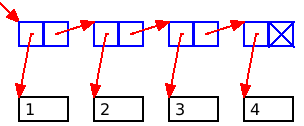
\includegraphics[width=0.5\textwidth]{simplelist}

\end{frame}
\sect{Scheme Programs are Lists}


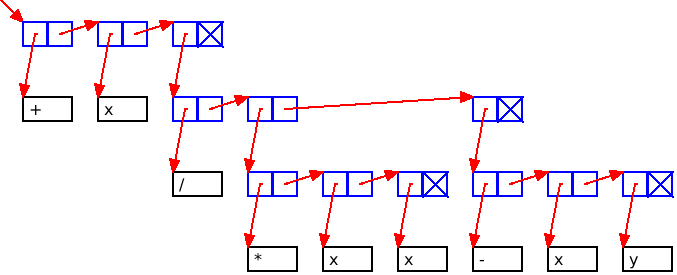
\includegraphics[width=\textwidth]{boxarrow}

\fbox{\tt (+ x (/ (* x x) (- x y)))}

\end{frame}

\sect{Building Lists in Scheme:}
\begin{enumerate}
\item The empty list in Scheme:  \fbox{\tt '()}
\item Create a list from 3 and the empty list: \fbox{\tt (cons 3 '()) $\Rightarrow$ (3)}
\item Create the list \fbox{\tt (4 7 2)}:
  \fbox{\tt (cons 4 (cons 7 (cons 2 '())))$\Rightarrow$ (4 7 2)}
\item Shorthand for long lists:
  \fbox{\tt (list 4 7 2)  $\Rightarrow$ (4 7 2)}
\pause
\item Using {\tt quote}:
  \fbox{\tt '(4 7 2)  $\Rightarrow$ (4 7 2)}\\
  \fbox{\tt '(+ 4 7 2)  $\Rightarrow$ (+ 4 7 2)}\\
  \fbox{\tt '(a b c) $\Rightarrow$ (a b c)}\\
  \fbox{\tt (a b c) $\Rightarrow$ {\em error}}\\
  \fbox{\tt (+ 4 7 2)  $\Rightarrow$ 13}\\
  \fbox{\tt '(list (+ 2 2) 7 2)  $\Rightarrow$ (list (+ 2 2) 7 2)}\\
  \fbox{\tt (list (+ 2 2) 7 2)  $\Rightarrow$ (4 7 2)}\\
  
\end{enumerate}

\end{frame}


\sect{An improper list results in a dot:}
\begin{itemize}
\item \fbox{\tt (cons 4 8) $\Rightarrow$ (4 . 8)}
\item \fbox{\tt (cons 3 (cons 5 (cons 7 9))) $\Rightarrow$ (3 5 7 . 9)}
\item Run {\tt boxarrow.rkt} for pictures.
\end{itemize}
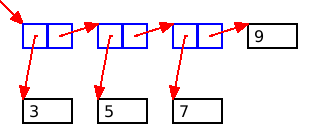
\includegraphics[width=0.5\textwidth]{improperlist}
\end{frame}

\sect{length}
\pause
\begin{Verbatim}
(define (length lst)
  (if (empty? lst)
      0
      (+ 1 (length (cdr lst)))))
\end{Verbatim}
\end{frame}
\sect{nth}
\pause
\begin{Verbatim}
(define (nth lst n)
  (cond ((empty? lst) '())
        ((= n 0) "Not defined")
        ((= n 1) (car lst))
        (else (nth (cdr lst) (- n 1)))))
\end{Verbatim}
\end{frame}
\sect{last}
\pause
\begin{Verbatim}
(define (last lst)
  (cond ((empty? lst) '())
        ((empty? (cdr lst)) (car lst))
        (else (last (cdr lst)))))
\end{Verbatim}
\end{frame}
\sect{scale-list}
\pause
\begin{Verbatim}
(define (scale-list lst n)
  (if (empty? lst)
      '()
      (cons (* n (car lst))
            (scale-list (cdr lst) n))))
\end{Verbatim}
\end{frame}
\sect{increment-list}
\pause
\begin{Verbatim}
(define (increment-list lst)
  (if (empty? lst)
      '()
      (cons (+ 1 (car lst))
            (increment-list (cdr lst)))))
\end{Verbatim}
\end{frame}
\sect{map}
\pause
\begin{Verbatim}
(define (map lst op)
  (if (empty? lst)
      '()
      (cons (op (car lst))
            (map (cdr lst) op))))
\end{Verbatim}
\end{frame}
\sect{scale-list using map}
\pause
\begin{Verbatim}
(define (scale-list lst n)
  (map lst (lambda (x) (* n x))))
\end{Verbatim}
\end{frame}
\sect{increment-list using map}
\pause
\begin{Verbatim}
(define (increment-list lst)
  (map lst (lambda (x) (+ x 1))))
\end{Verbatim}
\end{frame}
\sect{append}
\pause
\begin{Verbatim}
(define (append lst1 lst2)
  (if (empty? lst1)
      lst2
      (cons (car lst1)
            (append (cdr lst1) lst2))))
\end{Verbatim}
\end{frame}
\sect{remove}
\pause
\begin{Verbatim}
(define (remove n lst)
  (cond ((empty? lst) '())
        ((= n (car lst)) (remove n (cdr lst)))
        (else (cons (car lst)
                    (remove n (cdr lst))))))
\end{Verbatim}

\end{frame}
\end{document}
